\section{Single-board Heater System}
\label{sec:sbhs}
A single-board heater system, shown in Fig. \ref{fig:single-board},
is a lab-in-a-box setup suitable for performing numerous control
experiments.  It is has been designed with the following objectives:  
\begin{itemize}
\item It should have a small time constant that will allow completion
  of an experiment in a short time.  This will enable students to
  carry out a large number of experiments in a single afternoon,
  thereby studying in detail an aspect of control system design in a
  single laboratory session.
\item The speed of response should not be too fast either.  For
  example, some electrical engineering systems are so fast that
  sophisticated instruments are required to capture the trends.  We
  wanted a device in which, the measurements can be seen with naked
  eye, as it happens in industrial systems.  It could also demonstrate
  other measurement issues, such as, noise.
\item The device should be of low cost.  It should be affordable to
  most people even in developing countries.  This will allow extensive
  experimentation, even in unsupervised sessions.
\item If we can access this device through an open source software,
  the students trained in it will be attractive to the industry.
\end{itemize}

\subsection{Hardware}
The heater system, designed and developed at IIT Bombay, consists of a
heater assembly, fan, temperature sensor, microcontroller (ATmega16L)
and associated circuitry.  The functional block
diagram is shown in Fig. \ref{fig:block-heater}.

\begin{figure}
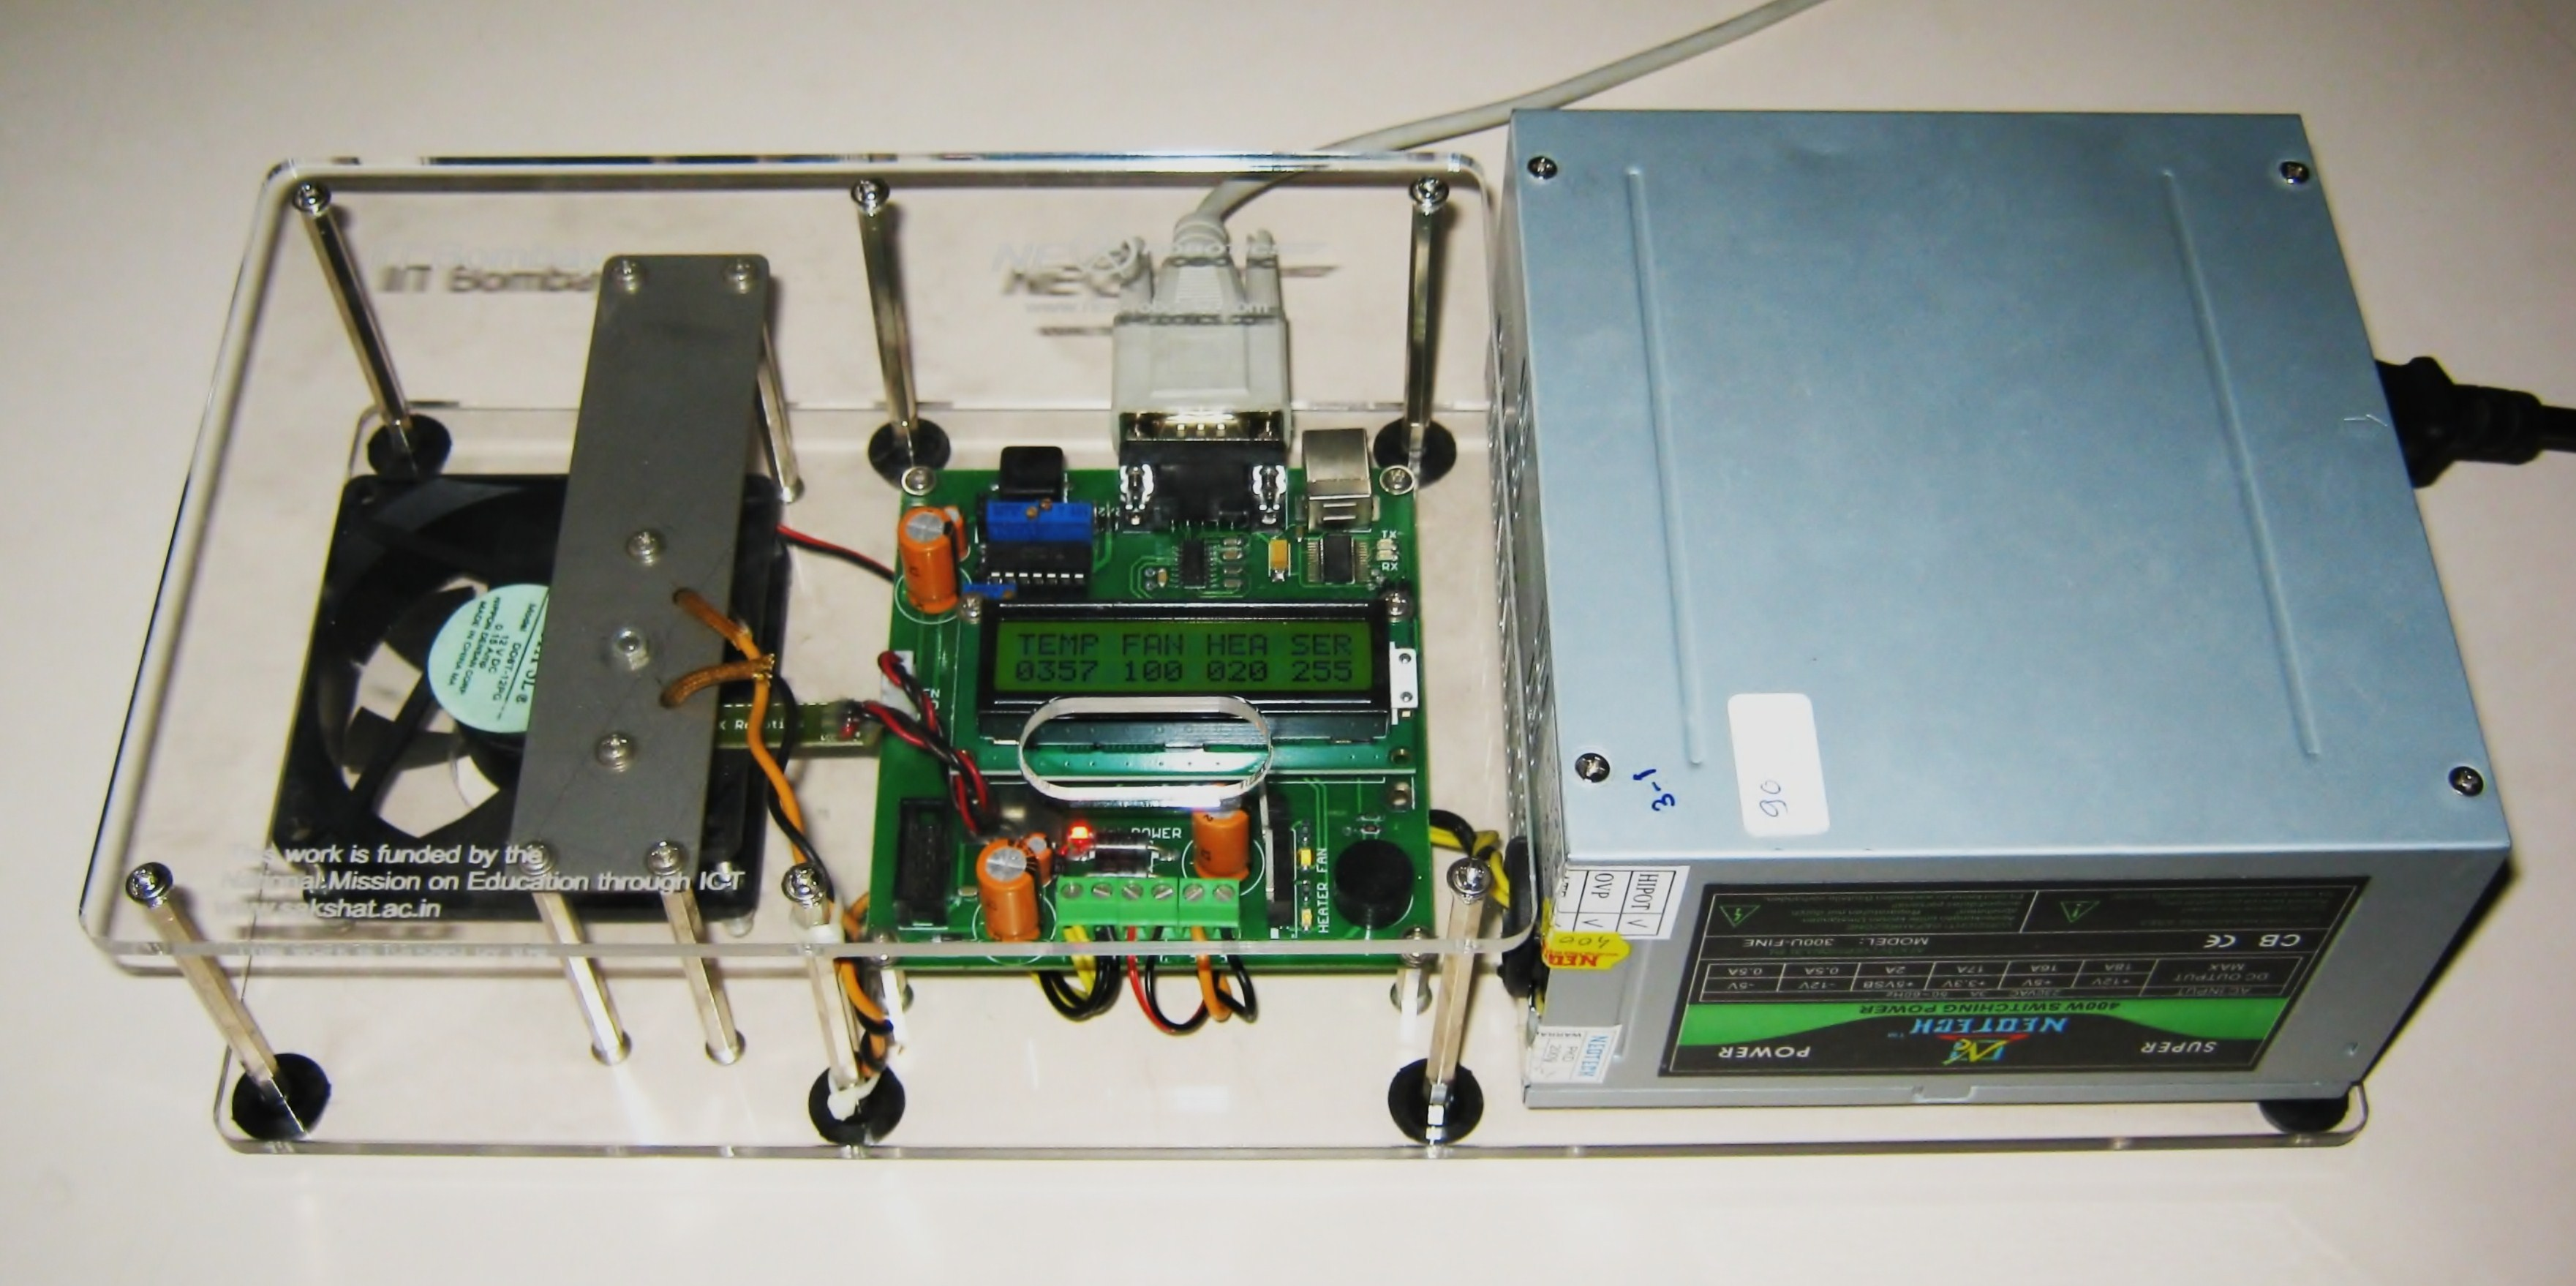
\includegraphics[width=\linewidth]{single-board.jpg}
\caption{Single-board heater system}
\label{fig:single-board}
\end{figure}

A stainless steel blade of size 5cm $\times$ 2cm, whose temperature
has to be controlled, serves as the plant.  Nichrome wire of 0.7mm
diameter, wound with 20 equally spaced helical turns into a coil of
5mm $\times$ 11mm and kept at a distance of 3.5mm from the steel
blade, acts as the heater element.  AD590, a monolithic integrated
circuit temperature transducer, is soldered beneath the steel plate.
AD590 is preferred over LM35 sensor that produces proportional voltage
output, because the latter gives erroneous readings even for small
connection resistances.  A computer fan, being a low cost and
commercially off the shelf component, is used to cool the plate from
below.

The temperature sensor produces linear current proportional to the
absolute temperature.  It produces 1 $\mu$A current per K.  The
corresponding voltage reading, in mV/K, taken across 1 k$\Omega$
resistor, is fed to an instrumentation amplifier having quad Opamp
LM324. The sensitivity is improved by operating ADC in 10-bit mode and
restricting the temperature range from 0 to $90^\circ C$. Maximum
possible resolution is then attained by subtracting 273 mV from the
sensor output followed by gain provision of 46.


% This
% system has signal conditioning circuitry at a physical distance of
% about 20 cm.  
% AD590 is rated to operate over a temperature range of
% -55 $^\circ$C to +150 $^\circ$C.  
% Metal package, TO-52, powered by
% LM1117-5V is used in the setup.

\begin{figure}
\centering
\includegraphics[width=\linewidth]{hea_31.pdf}
\caption{Functional block diagram}
\label{fig:block-heater}
\end{figure}

The microcontroller, ATmega16L, is the heart of this setup. It
converts analog temperature value to digital, serially communicates
command and data bytes with the computer, facilitates display of these
bytes on LCD and generates PWM wave to deliver proportional power to
the load.
%The setup is powered by an SMPS.

ATmega16L is an 8-bit AVR$\textcircled {R}$ microcontroller with an
advanced RISC architecture. Its on-chip programmable Flash, 4 PWM
channels, 8-channel 10-bit ADC, programmable serial Universal
Asynchronous Receiver and Transmitter(UART) and 32 general purpose
input and output lines make it suitable for this
application. Also, it is simple to program and readily available in
the local market.

The setup expends one ADC channel for the temperature sensor and two
PWM channels, one each, for heating assembly and fan. The remaining
ADC and PWM channels can well accommodate more sensors and load
respectively, thereby making the system versatile. 

An LCD mounted above the microcontroller, displays the temperature of
the heated plate, inputs to fan and heater, and also the commands
communicated via serial port.  The LCD, operated in 4-bit mode, uses
7-input/output lines of microcontroller for interface. The UART is
programmed to communicate at 9600 bps with the computer serial port.

ATmega16L supports clock speeds up to 16 MHz and processes most of the
instructions in one or two clock cycles. Since this application
doesn't need heavy processing, the system uses an on-chip oscillator
and an 8 MHz crystal.

% After current to voltage conversion, the sensor output is 1 mV per
% K. With ADC resolution of 4.88 mV per step, this corresponds to 4.8
% K.  By focusing on only the temperature range in the range of 0 to
% $90^\circ C$, the resolution is improved to one fourth.  However,
% the temperature of the heater plate is not expected to go below 0
% $^\circ$C. So the temperature below 273 K need not be
% measured. Also, the maximum temperature is restricted below 90
% $^\circ$C by the software. If 273 K is subtracted from the read
% temperature and the resultant is ampified such that 90 $^\circ$C
% represents 4.0 V(maximum that the opamp gives while operating at 5V)
% then the maximum possible resolution is obtained. Thus, before
% feeding the sensor output to the ADC of microcontroller, the
% subtraction by 273 mV, corresponding to 273 K, and amplification by
% a factor of 45 is done by quad Opamp LM324.  This, followed by
% amplification, is done by the quad Opamp LM324.

Each pin of the microcontroller can supply up to 30 mA of current
which is not sufficient to drive a heating element or a fan. To
increase the current driving capacity MOSFETs, IRFZ44
that can drive load up to 50 A, are used.

The setup has a provision for interfacing with either a serial or a
USB port of the computer. MAX232, a TTL-RS232 converter and FT232, a
USB-UART converter, respectively, take care of these. A jumper is
provided for the port selection.

This experimental setup is designed to operate at 12 V DC. The
microcontroller firmware limits the maximum current consumption to 1.6
A. If unlocked, the setup can draw up to 5 A. Computer SMPS, that can
deliver up to 8 A of current at 12 V DC, is used as a power
source, as it is cheaper, lighter and easier to handle, than a
transformer.

The setup is also provided with LM1117-5V low drop output voltage
regulator that supplies power to microcontroller, LCD, and TTL to
RS232 and USB to serial converters. Two 6A4 diodes are used for
protection against reverse polarity of load.


